% Options for packages loaded elsewhere
\PassOptionsToPackage{unicode}{hyperref}
\PassOptionsToPackage{hyphens}{url}
\documentclass[
  11pt,
]{article}
\usepackage{xcolor}
\usepackage[margin=1in]{geometry}
\usepackage{amsmath,amssymb}
\setcounter{secnumdepth}{5}
\usepackage{iftex}
\ifPDFTeX
  \usepackage[T1]{fontenc}
  \usepackage[utf8]{inputenc}
  \usepackage{textcomp} % provide euro and other symbols
\else % if luatex or xetex
  \usepackage{unicode-math} % this also loads fontspec
  \defaultfontfeatures{Scale=MatchLowercase}
  \defaultfontfeatures[\rmfamily]{Ligatures=TeX,Scale=1}
\fi
\usepackage{lmodern}
\ifPDFTeX\else
  % xetex/luatex font selection
\fi
% Use upquote if available, for straight quotes in verbatim environments
\IfFileExists{upquote.sty}{\usepackage{upquote}}{}
\IfFileExists{microtype.sty}{% use microtype if available
  \usepackage[]{microtype}
  \UseMicrotypeSet[protrusion]{basicmath} % disable protrusion for tt fonts
}{}
\makeatletter
\@ifundefined{KOMAClassName}{% if non-KOMA class
  \IfFileExists{parskip.sty}{%
    \usepackage{parskip}
  }{% else
    \setlength{\parindent}{0pt}
    \setlength{\parskip}{6pt plus 2pt minus 1pt}}
}{% if KOMA class
  \KOMAoptions{parskip=half}}
\makeatother
\usepackage{color}
\usepackage{fancyvrb}
\newcommand{\VerbBar}{|}
\newcommand{\VERB}{\Verb[commandchars=\\\{\}]}
\DefineVerbatimEnvironment{Highlighting}{Verbatim}{commandchars=\\\{\}}
% Add ',fontsize=\small' for more characters per line
\usepackage{framed}
\definecolor{shadecolor}{RGB}{248,248,248}
\newenvironment{Shaded}{\begin{snugshade}}{\end{snugshade}}
\newcommand{\AlertTok}[1]{\textcolor[rgb]{0.94,0.16,0.16}{#1}}
\newcommand{\AnnotationTok}[1]{\textcolor[rgb]{0.56,0.35,0.01}{\textbf{\textit{#1}}}}
\newcommand{\AttributeTok}[1]{\textcolor[rgb]{0.13,0.29,0.53}{#1}}
\newcommand{\BaseNTok}[1]{\textcolor[rgb]{0.00,0.00,0.81}{#1}}
\newcommand{\BuiltInTok}[1]{#1}
\newcommand{\CharTok}[1]{\textcolor[rgb]{0.31,0.60,0.02}{#1}}
\newcommand{\CommentTok}[1]{\textcolor[rgb]{0.56,0.35,0.01}{\textit{#1}}}
\newcommand{\CommentVarTok}[1]{\textcolor[rgb]{0.56,0.35,0.01}{\textbf{\textit{#1}}}}
\newcommand{\ConstantTok}[1]{\textcolor[rgb]{0.56,0.35,0.01}{#1}}
\newcommand{\ControlFlowTok}[1]{\textcolor[rgb]{0.13,0.29,0.53}{\textbf{#1}}}
\newcommand{\DataTypeTok}[1]{\textcolor[rgb]{0.13,0.29,0.53}{#1}}
\newcommand{\DecValTok}[1]{\textcolor[rgb]{0.00,0.00,0.81}{#1}}
\newcommand{\DocumentationTok}[1]{\textcolor[rgb]{0.56,0.35,0.01}{\textbf{\textit{#1}}}}
\newcommand{\ErrorTok}[1]{\textcolor[rgb]{0.64,0.00,0.00}{\textbf{#1}}}
\newcommand{\ExtensionTok}[1]{#1}
\newcommand{\FloatTok}[1]{\textcolor[rgb]{0.00,0.00,0.81}{#1}}
\newcommand{\FunctionTok}[1]{\textcolor[rgb]{0.13,0.29,0.53}{\textbf{#1}}}
\newcommand{\ImportTok}[1]{#1}
\newcommand{\InformationTok}[1]{\textcolor[rgb]{0.56,0.35,0.01}{\textbf{\textit{#1}}}}
\newcommand{\KeywordTok}[1]{\textcolor[rgb]{0.13,0.29,0.53}{\textbf{#1}}}
\newcommand{\NormalTok}[1]{#1}
\newcommand{\OperatorTok}[1]{\textcolor[rgb]{0.81,0.36,0.00}{\textbf{#1}}}
\newcommand{\OtherTok}[1]{\textcolor[rgb]{0.56,0.35,0.01}{#1}}
\newcommand{\PreprocessorTok}[1]{\textcolor[rgb]{0.56,0.35,0.01}{\textit{#1}}}
\newcommand{\RegionMarkerTok}[1]{#1}
\newcommand{\SpecialCharTok}[1]{\textcolor[rgb]{0.81,0.36,0.00}{\textbf{#1}}}
\newcommand{\SpecialStringTok}[1]{\textcolor[rgb]{0.31,0.60,0.02}{#1}}
\newcommand{\StringTok}[1]{\textcolor[rgb]{0.31,0.60,0.02}{#1}}
\newcommand{\VariableTok}[1]{\textcolor[rgb]{0.00,0.00,0.00}{#1}}
\newcommand{\VerbatimStringTok}[1]{\textcolor[rgb]{0.31,0.60,0.02}{#1}}
\newcommand{\WarningTok}[1]{\textcolor[rgb]{0.56,0.35,0.01}{\textbf{\textit{#1}}}}
\usepackage{graphicx}
\makeatletter
\newsavebox\pandoc@box
\newcommand*\pandocbounded[1]{% scales image to fit in text height/width
  \sbox\pandoc@box{#1}%
  \Gscale@div\@tempa{\textheight}{\dimexpr\ht\pandoc@box+\dp\pandoc@box\relax}%
  \Gscale@div\@tempb{\linewidth}{\wd\pandoc@box}%
  \ifdim\@tempb\p@<\@tempa\p@\let\@tempa\@tempb\fi% select the smaller of both
  \ifdim\@tempa\p@<\p@\scalebox{\@tempa}{\usebox\pandoc@box}%
  \else\usebox{\pandoc@box}%
  \fi%
}
% Set default figure placement to htbp
\def\fps@figure{htbp}
\makeatother
\setlength{\emergencystretch}{3em} % prevent overfull lines
\providecommand{\tightlist}{%
  \setlength{\itemsep}{0pt}\setlength{\parskip}{0pt}}
\usepackage{amsmath}
% Shared LaTeX preamble for all Data Mining / ISLR chapter documents.
% Provides \makecoverpage{<assignment title>} — a standalone title page
% with fixed student identity, so every chapter/lab looks uniform.

\usepackage{graphicx}

\newcommand{\makecoverpage}[1]{%
\begin{titlepage}
\centering
\vspace*{2cm}

{\Large \textbf{Adventist University of Central Africa}}\\[0.4cm]
{\large Master's in Big Data Analytics}\\[2cm]

{\Huge \textbf{#1}}\\[0.5cm]
{\large \textit{Introduction to Statistical Learning with Applications in R}}\\[3cm]

\begin{tabular}{rl}
\textbf{Programme:} & MSc Big Data Analytics \\
\textbf{Course Title:} & Data Mining \\
\textbf{Course Code:} & MSDA 9124 \\
\textbf{Lecturer:} & Dr. Pacifique Nizeyimana \\
\textbf{Student Name:} & Wayne Rubangisa \\
\textbf{Student ID:} & 101220 \\
\end{tabular}

\vfill

{\large September 2026}

\end{titlepage}
}

\usepackage{bookmark}
\IfFileExists{xurl.sty}{\usepackage{xurl}}{} % add URL line breaks if available
\urlstyle{same}
\hypersetup{
  hidelinks,
  pdfcreator={LaTeX via pandoc}}

\author{}
\date{\vspace{-2.5em}}

\begin{document}

\makecoverpage{Chapter 12 --- Unsupervised Learning \\ Exercises 4 and 11}

\begin{Shaded}
\begin{Highlighting}[]
\FunctionTok{library}\NormalTok{(ISLR2)}
\end{Highlighting}
\end{Shaded}

\section{Exercise 4: Single Linkage versus Complete
Linkage}\label{exercise-4-single-linkage-versus-complete-linkage}

Hierarchical clustering starts with every observation in its own cluster
and then repeatedly merges the two clusters that are closest according
to a chosen linkage rule. The linkage rule does not change the pairwise
distances between individual observations. It changes how we define the
distance between two \emph{clusters}.

For two clusters \(A\) and \(B\), single linkage uses the closest pair
of points:

\[
D_{\mathrm{single}}(A,B) = \min_{i\in A,\,j\in B} d(i,j).
\]

Complete linkage uses the farthest pair of points:

\[
D_{\mathrm{complete}}(A,B) = \max_{i\in A,\,j\in B} d(i,j).
\]

Because a maximum is always at least as large as a minimum,

\[
D_{\mathrm{complete}}(A,B) \geq D_{\mathrm{single}}(A,B)
\]

for every pair of clusters \(A\) and \(B\). This simple inequality is
the key to both parts of the exercise.

\subsection{\texorpdfstring{(a) The clusters \(\{1,2,3\}\) and
\(\{4,5\}\)}{(a) The clusters \textbackslash\{1,2,3\textbackslash\} and \textbackslash\{4,5\textbackslash\}}}\label{a-the-clusters-123-and-45}

The two methods merge the same two clusters at some point in their
respective dendrograms. The question is whether the fusion occurs
higher, at the same height, or whether there is not enough information
to tell.

The answer is that the complete-linkage fusion occurs \textbf{higher
than or at the same height as} the single-linkage fusion. It cannot
occur lower.

The reason is direct. For these particular clusters, write

\[
A=\{1,2,3\}, \qquad B=\{4,5\}.
\]

Then

\[
D_{\mathrm{single}}(A,B)
= \min\{d(1,4),d(1,5),d(2,4),d(2,5),d(3,4),d(3,5)\},
\]

whereas

\[
D_{\mathrm{complete}}(A,B)
= \max\{d(1,4),d(1,5),d(2,4),d(2,5),d(3,4),d(3,5)\}.
\]

The maximum is at least the minimum. Since dendrogram height records the
linkage distance at which a fusion occurs, the complete-linkage height
is at least the single-linkage height.

It is important to distinguish this conclusion from the stronger
statement that the heights must be different. They need not be. If all
six cross-cluster distances happen to be equal, then their minimum and
maximum are equal and both methods fuse the clusters at the same height.
Without the actual pairwise distances, we cannot decide whether the
inequality is strict.

Therefore, the precise answer is:

\[
\boxed{
\text{Complete linkage fuses }\{1,2,3\}\text{ and }\{4,5\}
\text{ at a height at least as large as single linkage.}
}
\]

\subsection{\texorpdfstring{(b) The clusters \(\{5\}\) and
\(\{6\}\)}{(b) The clusters \textbackslash\{5\textbackslash\} and \textbackslash\{6\textbackslash\}}}\label{b-the-clusters-5-and-6}

Here each cluster contains only one observation:

\[
A=\{5\}, \qquad B=\{6\}.
\]

There is only one cross-cluster distance, \(d(5,6)\). Therefore the
minimum and maximum over the set containing this one value are
identical:

\[
D_{\mathrm{single}}(\{5\},\{6\})
= d(5,6)
= D_{\mathrm{complete}}(\{5\},\{6\}).
\]

Consequently, the two methods fuse observations 5 and 6 at
\textbf{exactly the same height}.

This conclusion does not depend on the locations of observations 5 and 6
or on the rest of the dataset. Whenever both clusters are singletons,
every linkage definition based on the minimum or maximum of
cross-cluster distances reduces to the same one pairwise distance.

Thus,

\[
\boxed{
\text{The single-linkage and complete-linkage fusions occur at the same height.}
}
\]

\section{Exercise 11: Matrix
Completion}\label{exercise-11-matrix-completion}

Matrix completion estimates entries that are missing from a matrix by
using low-dimensional structure in the entries that are observed. The
central assumption is that the complete matrix is approximately low
rank. In other words, although the matrix may have many rows and
columns, most of its variation can be represented using a relatively
small number of latent components.

Suppose \(X\) is the unknown complete matrix and \(\Omega\) is the set
of observed entries. We observe \(X_{ij}\) only for \((i,j)\in\Omega\).
A rank-\(M\) approximation seeks a matrix \(\widehat X\) of the form

\[
\widehat X_M = U_M D_M V_M^T,
\]

where \(U_M\) and \(V_M\) contain the first \(M\) singular vectors and
\(D_M\) contains the first \(M\) singular values. Equivalently, the
singular value decomposition gives

\[
X \approx \sum_{m=1}^{M} d_m u_m v_m^T.
\]

Each outer product \(u_m v_m^T\) is a rank-one pattern. Increasing \(M\)
allows more patterns to be represented, so approximation bias generally
decreases; however, larger values of \(M\) can also fit noise and are
more expensive to estimate when many entries are missing.

\subsection{Algorithm 12.1 in plain
language}\label{algorithm-12.1-in-plain-language}

The matrix-completion algorithm alternates between two operations:

\begin{enumerate}
\def\labelenumi{\arabic{enumi}.}
\tightlist
\item
  fill the missing entries with current guesses;
\item
  compute a rank-\(M\) approximation of the completed matrix using the
  SVD, then use that approximation to update the missing entries.
\end{enumerate}

The observed entries are never changed. They anchor the procedure to the
actual data, while the unobserved entries are repeatedly replaced by
values consistent with the estimated low-rank structure.

Let \(P_\Omega\) be the projection that keeps observed entries and sets
missing entries to zero. The update can be written conceptually as

\[
X^{(t+1)}
= P_\Omega(X) + P_{\Omega^c}\left(\mathcal{P}_M(X^{(t)})\right),
\]

where \(\mathcal{P}_M\) means the best rank-\(M\) SVD approximation and
\(\Omega^c\) is the set of missing entries. The first term restores the
observed values; the second supplies estimates only where values are
missing.

The function below also tracks a convergence quantity. After each
update, it computes the relative change between consecutive completed
matrices:

\[
\delta_t =
\frac{\left\|X^{(t+1)}-X^{(t)}\right\|_F}
{\max\left(\left\|X^{(t)}\right\|_F,\varepsilon\right)},
\]

where \(\|\cdot\|_F\) is the Frobenius norm and \(\varepsilon\) prevents
division by zero. Iteration stops when \(\delta_t\) is below
\texttt{tol} or when \texttt{max\_iter} is reached.

\begin{Shaded}
\begin{Highlighting}[]
\NormalTok{rank\_m\_approximation }\OtherTok{\textless{}{-}} \ControlFlowTok{function}\NormalTok{(x, M) \{}
\NormalTok{  decomposition }\OtherTok{\textless{}{-}} \FunctionTok{svd}\NormalTok{(x, }\AttributeTok{nu =}\NormalTok{ M, }\AttributeTok{nv =}\NormalTok{ M)}
\NormalTok{  rank\_used }\OtherTok{\textless{}{-}} \FunctionTok{min}\NormalTok{(M, }\FunctionTok{length}\NormalTok{(decomposition}\SpecialCharTok{$}\NormalTok{d))}

\NormalTok{  decomposition}\SpecialCharTok{$}\NormalTok{u[, }\FunctionTok{seq\_len}\NormalTok{(rank\_used), drop }\OtherTok{=} \ConstantTok{FALSE}\NormalTok{] }\SpecialCharTok{\%*\%}
\NormalTok{    (decomposition}\SpecialCharTok{$}\NormalTok{d[}\FunctionTok{seq\_len}\NormalTok{(rank\_used)] }\SpecialCharTok{*}
       \FunctionTok{t}\NormalTok{(decomposition}\SpecialCharTok{$}\NormalTok{v[, }\FunctionTok{seq\_len}\NormalTok{(rank\_used), }\AttributeTok{drop =} \ConstantTok{FALSE}\NormalTok{]))}
\NormalTok{\}}

\NormalTok{matrix\_completion }\OtherTok{\textless{}{-}} \ControlFlowTok{function}\NormalTok{(X\_observed,}
\NormalTok{                              observed,}
\NormalTok{                              M,}
                              \AttributeTok{tol =} \FloatTok{1e{-}5}\NormalTok{,}
                              \AttributeTok{max\_iter =} \DecValTok{1000}\NormalTok{,}
                              \AttributeTok{verbose =} \ConstantTok{FALSE}\NormalTok{) \{}
  \FunctionTok{stopifnot}\NormalTok{(}\FunctionTok{is.matrix}\NormalTok{(X\_observed), }\FunctionTok{is.matrix}\NormalTok{(observed))}
  \FunctionTok{stopifnot}\NormalTok{(}\FunctionTok{all}\NormalTok{(}\FunctionTok{dim}\NormalTok{(X\_observed) }\SpecialCharTok{==} \FunctionTok{dim}\NormalTok{(observed)))}
  \FunctionTok{stopifnot}\NormalTok{(}\FunctionTok{length}\NormalTok{(M) }\SpecialCharTok{==} \DecValTok{1}\NormalTok{, M }\SpecialCharTok{\textgreater{}=} \DecValTok{1}\NormalTok{, M }\SpecialCharTok{==} \FunctionTok{as.integer}\NormalTok{(M))}
  \FunctionTok{stopifnot}\NormalTok{(}\FunctionTok{length}\NormalTok{(tol) }\SpecialCharTok{==} \DecValTok{1}\NormalTok{, tol }\SpecialCharTok{\textgreater{}} \DecValTok{0}\NormalTok{)}
  \FunctionTok{stopifnot}\NormalTok{(}\FunctionTok{length}\NormalTok{(max\_iter) }\SpecialCharTok{==} \DecValTok{1}\NormalTok{, max\_iter }\SpecialCharTok{\textgreater{}=} \DecValTok{1}\NormalTok{)}

  \ControlFlowTok{if}\NormalTok{ (}\SpecialCharTok{!}\FunctionTok{all}\NormalTok{(}\FunctionTok{is.finite}\NormalTok{(X\_observed[observed]))) \{}
    \FunctionTok{stop}\NormalTok{(}\StringTok{"Observed entries must be finite."}\NormalTok{)}
\NormalTok{  \}}
  \ControlFlowTok{if}\NormalTok{ (}\SpecialCharTok{!}\FunctionTok{any}\NormalTok{(observed)) \{}
    \FunctionTok{stop}\NormalTok{(}\StringTok{"At least one entry must be observed."}\NormalTok{)}
\NormalTok{  \}}

  \CommentTok{\# Column means provide a stable starting value for each missing entry.}
\NormalTok{  completed }\OtherTok{\textless{}{-}}\NormalTok{ X\_observed}
  \ControlFlowTok{for}\NormalTok{ (j }\ControlFlowTok{in} \FunctionTok{seq\_len}\NormalTok{(}\FunctionTok{ncol}\NormalTok{(completed))) \{}
\NormalTok{    observed\_in\_column }\OtherTok{\textless{}{-}}\NormalTok{ observed[, j]}
\NormalTok{    column\_mean }\OtherTok{\textless{}{-}} \ControlFlowTok{if}\NormalTok{ (}\FunctionTok{any}\NormalTok{(observed\_in\_column)) \{}
      \FunctionTok{mean}\NormalTok{(X\_observed[observed\_in\_column, j])}
\NormalTok{    \} }\ControlFlowTok{else}\NormalTok{ \{}
      \FunctionTok{mean}\NormalTok{(X\_observed[observed], }\AttributeTok{na.rm =} \ConstantTok{TRUE}\NormalTok{)}
\NormalTok{    \}}
\NormalTok{    completed[}\SpecialCharTok{!}\NormalTok{observed\_in\_column, j] }\OtherTok{\textless{}{-}}\NormalTok{ column\_mean}
\NormalTok{  \}}
\NormalTok{  completed[observed] }\OtherTok{\textless{}{-}}\NormalTok{ X\_observed[observed]}

\NormalTok{  convergence }\OtherTok{\textless{}{-}} \FunctionTok{numeric}\NormalTok{(max\_iter)}
\NormalTok{  approximation }\OtherTok{\textless{}{-}}\NormalTok{ completed}
\NormalTok{  iteration }\OtherTok{\textless{}{-}} \DecValTok{0}\DataTypeTok{L}

  \ControlFlowTok{for}\NormalTok{ (step }\ControlFlowTok{in} \FunctionTok{seq\_len}\NormalTok{(max\_iter)) \{}
\NormalTok{    approximation }\OtherTok{\textless{}{-}} \FunctionTok{rank\_m\_approximation}\NormalTok{(completed, M)}
\NormalTok{    updated }\OtherTok{\textless{}{-}}\NormalTok{ completed}
\NormalTok{    updated[}\SpecialCharTok{!}\NormalTok{observed] }\OtherTok{\textless{}{-}}\NormalTok{ approximation[}\SpecialCharTok{!}\NormalTok{observed]}
\NormalTok{    updated[observed] }\OtherTok{\textless{}{-}}\NormalTok{ X\_observed[observed]}

\NormalTok{    relative\_change }\OtherTok{\textless{}{-}} \FunctionTok{sqrt}\NormalTok{(}\FunctionTok{sum}\NormalTok{((updated }\SpecialCharTok{{-}}\NormalTok{ completed)}\SpecialCharTok{\^{}}\DecValTok{2}\NormalTok{)) }\SpecialCharTok{/}
      \FunctionTok{max}\NormalTok{(}\FunctionTok{sqrt}\NormalTok{(}\FunctionTok{sum}\NormalTok{(completed}\SpecialCharTok{\^{}}\DecValTok{2}\NormalTok{)), .Machine}\SpecialCharTok{$}\NormalTok{double.eps)}
\NormalTok{    convergence[step] }\OtherTok{\textless{}{-}}\NormalTok{ relative\_change}
\NormalTok{    iteration }\OtherTok{\textless{}{-}}\NormalTok{ step}

    \ControlFlowTok{if}\NormalTok{ (verbose) \{}
      \FunctionTok{cat}\NormalTok{(}\FunctionTok{sprintf}\NormalTok{(}\StringTok{"iteration \%d: relative change = \%.7g}\SpecialCharTok{\textbackslash{}n}\StringTok{"}\NormalTok{,}
\NormalTok{                  step, relative\_change))}
\NormalTok{    \}}

\NormalTok{    completed }\OtherTok{\textless{}{-}}\NormalTok{ updated}
    \ControlFlowTok{if}\NormalTok{ (relative\_change }\SpecialCharTok{\textless{}}\NormalTok{ tol) \{}
      \ControlFlowTok{break}
\NormalTok{    \}}
\NormalTok{  \}}

  \FunctionTok{list}\NormalTok{(}
    \AttributeTok{completed =}\NormalTok{ completed,}
    \AttributeTok{iterations =}\NormalTok{ iteration,}
    \AttributeTok{convergence =}\NormalTok{ convergence[}\FunctionTok{seq\_len}\NormalTok{(iteration)],}
    \AttributeTok{converged =}\NormalTok{ convergence[iteration] }\SpecialCharTok{\textless{}}\NormalTok{ tol,}
    \AttributeTok{rank =}\NormalTok{ M}
\NormalTok{  )}
\NormalTok{\}}
\end{Highlighting}
\end{Shaded}

The observed-entry constraint is worth checking explicitly. Even after
many iterations, the returned matrix must reproduce every value that was
supplied to the function:

\begin{Shaded}
\begin{Highlighting}[]
\FunctionTok{set.seed}\NormalTok{(}\DecValTok{12}\NormalTok{)}
\NormalTok{toy }\OtherTok{\textless{}{-}} \FunctionTok{matrix}\NormalTok{(}\FunctionTok{rnorm}\NormalTok{(}\DecValTok{30}\NormalTok{), }\AttributeTok{nrow =} \DecValTok{6}\NormalTok{)}
\NormalTok{toy\_observed }\OtherTok{\textless{}{-}} \FunctionTok{matrix}\NormalTok{(}\FunctionTok{runif}\NormalTok{(}\FunctionTok{length}\NormalTok{(toy)) }\SpecialCharTok{\textgreater{}} \FloatTok{0.25}\NormalTok{,}
                       \AttributeTok{nrow =} \FunctionTok{nrow}\NormalTok{(toy), }\AttributeTok{ncol =} \FunctionTok{ncol}\NormalTok{(toy))}
\NormalTok{toy\_input }\OtherTok{\textless{}{-}}\NormalTok{ toy}
\NormalTok{toy\_input[}\SpecialCharTok{!}\NormalTok{toy\_observed] }\OtherTok{\textless{}{-}} \ConstantTok{NA\_real\_}

\NormalTok{toy\_fit }\OtherTok{\textless{}{-}} \FunctionTok{matrix\_completion}\NormalTok{(toy\_input, toy\_observed, }\AttributeTok{M =} \DecValTok{2}\NormalTok{)}

\NormalTok{max\_observed\_difference }\OtherTok{\textless{}{-}} \FunctionTok{max}\NormalTok{(}\FunctionTok{abs}\NormalTok{(}
\NormalTok{  toy\_fit}\SpecialCharTok{$}\NormalTok{completed[toy\_observed] }\SpecialCharTok{{-}}\NormalTok{ toy[toy\_observed]}
\NormalTok{))}
\NormalTok{max\_observed\_difference}
\end{Highlighting}
\end{Shaded}

\begin{verbatim}
## [1] 0
\end{verbatim}

The maximum difference should be zero up to floating-point precision.
This check matters because a method that changes observed entries would
no longer be completing the matrix; it would simply be fitting a
low-rank approximation to a modified dataset.

\subsection{\texorpdfstring{Preparing the \texttt{Boston}
experiment}{Preparing the Boston experiment}}\label{preparing-the-boston-experiment}

The \texttt{Boston} dataset contains 506 observations and 13 numeric
features. The exercise asks us to standardize the features first. For
every feature \(j\), the transformation is

\[
Z_{ij} = \frac{X_{ij}-\bar X_j}{s_j},
\]

so each column has mean approximately zero and standard deviation one.
This is important because the SVD is scale-sensitive: without
standardization, a feature measured in large units could dominate the
decomposition simply because of its units rather than because it carries
more structure.

\begin{Shaded}
\begin{Highlighting}[]
\NormalTok{Boston\_features }\OtherTok{\textless{}{-}} \FunctionTok{as.matrix}\NormalTok{(ISLR2}\SpecialCharTok{::}\NormalTok{Boston[, }\FunctionTok{setdiff}\NormalTok{(}\FunctionTok{names}\NormalTok{(ISLR2}\SpecialCharTok{::}\NormalTok{Boston), }\StringTok{"medv"}\NormalTok{)])}
\NormalTok{Boston\_scaled }\OtherTok{\textless{}{-}} \FunctionTok{scale}\NormalTok{(Boston\_features)}

\FunctionTok{c}\NormalTok{(}
  \AttributeTok{largest\_absolute\_column\_mean =} \FunctionTok{max}\NormalTok{(}\FunctionTok{abs}\NormalTok{(}\FunctionTok{colMeans}\NormalTok{(Boston\_scaled))),}
  \AttributeTok{largest\_standard\_deviation\_error =} \FunctionTok{max}\NormalTok{(}\FunctionTok{abs}\NormalTok{(}\FunctionTok{apply}\NormalTok{(Boston\_scaled, }\DecValTok{2}\NormalTok{, sd) }\SpecialCharTok{{-}} \DecValTok{1}\NormalTok{))}
\NormalTok{)}
\end{Highlighting}
\end{Shaded}

\begin{verbatim}
##     largest_absolute_column_mean largest_standard_deviation_error 
##                     1.149882e-14                     8.215650e-15
\end{verbatim}

We evaluate approximation error only on entries that were deliberately
hidden. Because the original \texttt{Boston\_scaled} matrix is available
to us in this experiment, we can compare an imputed value with its known
truth. For a mask \(H\) of hidden entries, the relative error is

\[
\operatorname{RelErr}(\widehat X)
= \frac{\|H\odot(\widehat X-X)\|_F}
{\|H\odot X\|_F},
\]

where \(\odot\) denotes elementwise multiplication. Evaluating on hidden
entries is the matrix-completion analogue of using a test set: those
values were not supplied to the algorithm.

\subsection{One worked run}\label{one-worked-run}

This first run hides 15\% of the entries, uses a rank-\(M=3\)
approximation, and prints the convergence progress. The hidden entries
are created from a random permutation, so the missingness is random
while still allowing us to construct nested masks for the full
experiment below.

\begin{Shaded}
\begin{Highlighting}[]
\NormalTok{relative\_error }\OtherTok{\textless{}{-}} \ControlFlowTok{function}\NormalTok{(estimate, truth, hidden) \{}
  \FunctionTok{sqrt}\NormalTok{(}\FunctionTok{sum}\NormalTok{((estimate[hidden] }\SpecialCharTok{{-}}\NormalTok{ truth[hidden])}\SpecialCharTok{\^{}}\DecValTok{2}\NormalTok{)) }\SpecialCharTok{/}
    \FunctionTok{max}\NormalTok{(}\FunctionTok{sqrt}\NormalTok{(}\FunctionTok{sum}\NormalTok{(truth[hidden]}\SpecialCharTok{\^{}}\DecValTok{2}\NormalTok{)), .Machine}\SpecialCharTok{$}\NormalTok{double.eps)}
\NormalTok{\}}

\FunctionTok{set.seed}\NormalTok{(}\DecValTok{11}\NormalTok{)}
\NormalTok{missing\_fraction }\OtherTok{\textless{}{-}} \FloatTok{0.15}
\NormalTok{hidden\_count }\OtherTok{\textless{}{-}} \FunctionTok{ceiling}\NormalTok{(missing\_fraction }\SpecialCharTok{*} \FunctionTok{length}\NormalTok{(Boston\_scaled))}
\NormalTok{hidden\_indices }\OtherTok{\textless{}{-}} \FunctionTok{sample}\NormalTok{(}\FunctionTok{seq\_along}\NormalTok{(Boston\_scaled), hidden\_count)}
\NormalTok{hidden }\OtherTok{\textless{}{-}} \FunctionTok{matrix}\NormalTok{(}\ConstantTok{FALSE}\NormalTok{, }\FunctionTok{nrow}\NormalTok{(Boston\_scaled), }\FunctionTok{ncol}\NormalTok{(Boston\_scaled))}
\NormalTok{hidden[hidden\_indices] }\OtherTok{\textless{}{-}} \ConstantTok{TRUE}
\NormalTok{observed }\OtherTok{\textless{}{-}} \SpecialCharTok{!}\NormalTok{hidden}

\NormalTok{input }\OtherTok{\textless{}{-}}\NormalTok{ Boston\_scaled}
\NormalTok{input[hidden] }\OtherTok{\textless{}{-}} \ConstantTok{NA\_real\_}
\NormalTok{worked\_run }\OtherTok{\textless{}{-}} \FunctionTok{matrix\_completion}\NormalTok{(input, observed, }\AttributeTok{M =} \DecValTok{3}\NormalTok{,}
                                \AttributeTok{tol =} \FloatTok{1e{-}5}\NormalTok{, }\AttributeTok{max\_iter =} \DecValTok{500}\NormalTok{,}
                                \AttributeTok{verbose =} \ConstantTok{TRUE}\NormalTok{)}
\end{Highlighting}
\end{Shaded}

\begin{verbatim}
## iteration 1: relative change = 0.2397423
## iteration 2: relative change = 0.07734169
## iteration 3: relative change = 0.03435819
## iteration 4: relative change = 0.01913215
## iteration 5: relative change = 0.01216897
## iteration 6: relative change = 0.008320287
## iteration 7: relative change = 0.005921288
## iteration 8: relative change = 0.0043143
## iteration 9: relative change = 0.003190163
## iteration 10: relative change = 0.002382493
## iteration 11: relative change = 0.001792249
## iteration 12: relative change = 0.001356022
## iteration 13: relative change = 0.001031114
## iteration 14: relative change = 0.0007877646
## iteration 15: relative change = 0.0006047486
## iteration 16: relative change = 0.0004666875
## iteration 17: relative change = 0.0003623133
## iteration 18: relative change = 0.0002832998
## iteration 19: relative change = 0.0002234514
## iteration 20: relative change = 0.0001781273
## iteration 21: relative change = 0.0001438272
## iteration 22: relative change = 0.0001178911
## iteration 23: relative change = 9.828156e-05
## iteration 24: relative change = 8.342855e-05
## iteration 25: relative change = 7.212053e-05
## iteration 26: relative change = 6.342747e-05
## iteration 27: relative change = 5.664452e-05
## iteration 28: relative change = 5.124706e-05
## iteration 29: relative change = 4.685232e-05
## iteration 30: relative change = 4.318618e-05
## iteration 31: relative change = 4.005516e-05
## iteration 32: relative change = 3.732396e-05
## iteration 33: relative change = 3.489828e-05
## iteration 34: relative change = 3.271229e-05
## iteration 35: relative change = 3.071963e-05
## iteration 36: relative change = 2.888724e-05
## iteration 37: relative change = 2.719109e-05
## iteration 38: relative change = 2.561334e-05
## iteration 39: relative change = 2.41404e-05
## iteration 40: relative change = 2.27616e-05
## iteration 41: relative change = 2.146835e-05
## iteration 42: relative change = 2.025355e-05
## iteration 43: relative change = 1.911116e-05
## iteration 44: relative change = 1.803597e-05
## iteration 45: relative change = 1.702337e-05
## iteration 46: relative change = 1.606925e-05
## iteration 47: relative change = 1.516987e-05
## iteration 48: relative change = 1.432183e-05
## iteration 49: relative change = 1.3522e-05
## iteration 50: relative change = 1.27675e-05
## iteration 51: relative change = 1.205562e-05
## iteration 52: relative change = 1.138387e-05
## iteration 53: relative change = 1.074991e-05
## iteration 54: relative change = 1.015156e-05
## iteration 55: relative change = 9.586762e-06
\end{verbatim}

\begin{Shaded}
\begin{Highlighting}[]
\FunctionTok{list}\NormalTok{(}
  \AttributeTok{iterations =}\NormalTok{ worked\_run}\SpecialCharTok{$}\NormalTok{iterations,}
  \AttributeTok{converged =}\NormalTok{ worked\_run}\SpecialCharTok{$}\NormalTok{converged,}
  \AttributeTok{final\_relative\_change =} \FunctionTok{tail}\NormalTok{(worked\_run}\SpecialCharTok{$}\NormalTok{convergence, }\DecValTok{1}\NormalTok{),}
  \AttributeTok{hidden\_entry\_relative\_error =} \FunctionTok{relative\_error}\NormalTok{(}
\NormalTok{    worked\_run}\SpecialCharTok{$}\NormalTok{completed, Boston\_scaled, hidden}
\NormalTok{  )}
\NormalTok{)}
\end{Highlighting}
\end{Shaded}

\begin{verbatim}
## $iterations
## [1] 55
## 
## $converged
## [1] TRUE
## 
## $final_relative_change
## [1] 9.586762e-06
## 
## $hidden_entry_relative_error
## [1] 0.7695113
\end{verbatim}

The convergence value and the approximation error answer different
questions. The convergence value asks whether successive imputations
have stopped changing. The hidden-entry error asks whether the final
imputations are close to the values that were actually hidden.
Convergence is necessary for a stable iteration, but it does not by
itself guarantee a small prediction error.

\subsection{Nested missingness
experiment}\label{nested-missingness-experiment}

We now follow the exercise exactly. The missing fractions are 5\%, 10\%,
\ldots, 30\%. For each of 10 repetitions, one random ordering of all
matrix entries is created. The first 5\% of that ordering are hidden for
the 5\% experiment, the first 10\% are hidden for the 10\% experiment,
and so on. Thus the missing sets are nested within each repetition.

For every missingness level and every \(M\in\{1,2,\ldots,8\}\), we run
the completion algorithm and calculate the hidden-entry relative error.

\begin{Shaded}
\begin{Highlighting}[]
\FunctionTok{set.seed}\NormalTok{(}\DecValTok{2026}\NormalTok{)}
\NormalTok{missing\_fractions }\OtherTok{\textless{}{-}} \FunctionTok{seq}\NormalTok{(}\FloatTok{0.05}\NormalTok{, }\FloatTok{0.30}\NormalTok{, }\AttributeTok{by =} \FloatTok{0.05}\NormalTok{)}
\NormalTok{rank\_values }\OtherTok{\textless{}{-}} \DecValTok{1}\SpecialCharTok{:}\DecValTok{8}
\NormalTok{repetitions }\OtherTok{\textless{}{-}} \DecValTok{10}

\NormalTok{experiment\_results }\OtherTok{\textless{}{-}} \FunctionTok{vector}\NormalTok{(}\StringTok{"list"}\NormalTok{, }\FunctionTok{length}\NormalTok{(missing\_fractions) }\SpecialCharTok{*}
                               \FunctionTok{length}\NormalTok{(rank\_values) }\SpecialCharTok{*}\NormalTok{ repetitions)}
\NormalTok{result\_index }\OtherTok{\textless{}{-}} \DecValTok{1}\DataTypeTok{L}

\ControlFlowTok{for}\NormalTok{ (replication }\ControlFlowTok{in} \FunctionTok{seq\_len}\NormalTok{(repetitions)) \{}
\NormalTok{  permutation }\OtherTok{\textless{}{-}} \FunctionTok{sample}\NormalTok{(}\FunctionTok{seq\_along}\NormalTok{(Boston\_scaled))}

  \ControlFlowTok{for}\NormalTok{ (missing\_fraction }\ControlFlowTok{in}\NormalTok{ missing\_fractions) \{}
\NormalTok{    hidden\_count }\OtherTok{\textless{}{-}} \FunctionTok{ceiling}\NormalTok{(missing\_fraction }\SpecialCharTok{*} \FunctionTok{length}\NormalTok{(Boston\_scaled))}
\NormalTok{    hidden }\OtherTok{\textless{}{-}} \FunctionTok{matrix}\NormalTok{(}\ConstantTok{FALSE}\NormalTok{, }\FunctionTok{nrow}\NormalTok{(Boston\_scaled), }\FunctionTok{ncol}\NormalTok{(Boston\_scaled))}
\NormalTok{    hidden[permutation[}\FunctionTok{seq\_len}\NormalTok{(hidden\_count)]] }\OtherTok{\textless{}{-}} \ConstantTok{TRUE}
\NormalTok{    observed }\OtherTok{\textless{}{-}} \SpecialCharTok{!}\NormalTok{hidden}

\NormalTok{    input }\OtherTok{\textless{}{-}}\NormalTok{ Boston\_scaled}
\NormalTok{    input[hidden] }\OtherTok{\textless{}{-}} \ConstantTok{NA\_real\_}

    \ControlFlowTok{for}\NormalTok{ (M }\ControlFlowTok{in}\NormalTok{ rank\_values) \{}
\NormalTok{      fit }\OtherTok{\textless{}{-}} \FunctionTok{matrix\_completion}\NormalTok{(input, observed, }\AttributeTok{M =}\NormalTok{ M,}
                               \AttributeTok{tol =} \FloatTok{1e{-}5}\NormalTok{, }\AttributeTok{max\_iter =} \DecValTok{500}\NormalTok{)}

\NormalTok{      experiment\_results[[result\_index]] }\OtherTok{\textless{}{-}} \FunctionTok{data.frame}\NormalTok{(}
        \AttributeTok{repetition =}\NormalTok{ replication,}
        \AttributeTok{missing\_fraction =}\NormalTok{ missing\_fraction,}
        \AttributeTok{M =}\NormalTok{ M,}
        \AttributeTok{approximation\_error =} \FunctionTok{relative\_error}\NormalTok{(}
\NormalTok{          fit}\SpecialCharTok{$}\NormalTok{completed, Boston\_scaled, hidden}
\NormalTok{        ),}
        \AttributeTok{iterations =}\NormalTok{ fit}\SpecialCharTok{$}\NormalTok{iterations,}
        \AttributeTok{converged =}\NormalTok{ fit}\SpecialCharTok{$}\NormalTok{converged}
\NormalTok{      )}
\NormalTok{      result\_index }\OtherTok{\textless{}{-}}\NormalTok{ result\_index }\SpecialCharTok{+} \DecValTok{1}\DataTypeTok{L}
\NormalTok{    \}}
\NormalTok{  \}}
\NormalTok{\}}

\NormalTok{experiment\_results }\OtherTok{\textless{}{-}} \FunctionTok{do.call}\NormalTok{(rbind, experiment\_results)}
\FunctionTok{head}\NormalTok{(experiment\_results)}
\end{Highlighting}
\end{Shaded}

\begin{verbatim}
##   repetition missing_fraction M approximation_error iterations converged
## 1          1             0.05 1           0.7433034          9      TRUE
## 2          1             0.05 2           0.7516467         13      TRUE
## 3          1             0.05 3           0.7270391         16      TRUE
## 4          1             0.05 4           1.6350666        500     FALSE
## 5          1             0.05 5           1.7487664        500     FALSE
## 6          1             0.05 6           1.7616430        500     FALSE
\end{verbatim}

\subsection{Average approximation
error}\label{average-approximation-error}

\begin{Shaded}
\begin{Highlighting}[]
\NormalTok{error\_summary }\OtherTok{\textless{}{-}} \FunctionTok{aggregate}\NormalTok{(}
\NormalTok{  approximation\_error }\SpecialCharTok{\textasciitilde{}}\NormalTok{ missing\_fraction }\SpecialCharTok{+}\NormalTok{ M,}
  \AttributeTok{data =}\NormalTok{ experiment\_results,}
  \AttributeTok{FUN =}\NormalTok{ mean}
\NormalTok{)}
\NormalTok{error\_summary}
\end{Highlighting}
\end{Shaded}

\begin{verbatim}
##    missing_fraction M approximation_error
## 1              0.05 1           0.7662636
## 2              0.10 1           0.7687960
## 3              0.15 1           0.7737457
## 4              0.20 1           0.7779226
## 5              0.25 1           0.7822767
## 6              0.30 1           0.7828148
## 7              0.05 2           0.7581456
## 8              0.10 2           0.7637368
## 9              0.15 2           0.7799377
## 10             0.20 2           0.8033937
## 11             0.25 2           0.8165775
## 12             0.30 2           0.8343027
## 13             0.05 3           0.7379708
## 14             0.10 3           0.7524522
## 15             0.15 3           0.7854768
## 16             0.20 3           0.8336620
## 17             0.25 3           0.8749093
## 18             0.30 3           0.9949447
## 19             0.05 4           1.7498005
## 20             0.10 4           1.6564260
## 21             0.15 4           1.6482757
## 22             0.20 4           1.6551721
## 23             0.25 4           1.4300589
## 24             0.30 4           1.5397663
## 25             0.05 5           1.9430449
## 26             0.10 5           1.8863537
## 27             0.15 5           1.9310998
## 28             0.20 5           1.9883614
## 29             0.25 5           1.9311053
## 30             0.30 5           1.8999691
## 31             0.05 6           2.1594985
## 32             0.10 6           2.0696658
## 33             0.15 6           2.0094303
## 34             0.20 6           2.0588072
## 35             0.25 6           2.0335435
## 36             0.30 6           1.9541001
## 37             0.05 7           2.1272487
## 38             0.10 7           2.0804777
## 39             0.15 7           2.0266779
## 40             0.20 7           2.1022470
## 41             0.25 7           2.0694801
## 42             0.30 7           1.9422833
## 43             0.05 8           2.2791991
## 44             0.10 8           2.1793132
## 45             0.15 8           2.1406799
## 46             0.20 8           2.0766689
## 47             0.25 8           1.9487890
## 48             0.30 8           1.7681085
\end{verbatim}

\begin{Shaded}
\begin{Highlighting}[]
\FunctionTok{plot}\NormalTok{(}\ConstantTok{NA}\NormalTok{, }\AttributeTok{xlim =} \FunctionTok{range}\NormalTok{(missing\_fractions),}
     \AttributeTok{ylim =} \FunctionTok{range}\NormalTok{(error\_summary}\SpecialCharTok{$}\NormalTok{approximation\_error),}
     \AttributeTok{xlab =} \StringTok{"Fraction of observations missing"}\NormalTok{,}
     \AttributeTok{ylab =} \StringTok{"Mean relative approximation error"}\NormalTok{,}
     \AttributeTok{main =} \StringTok{"Matrix{-}completion error across missingness and rank"}\NormalTok{)}

\ControlFlowTok{for}\NormalTok{ (M }\ControlFlowTok{in}\NormalTok{ rank\_values) \{}
\NormalTok{  curve\_data }\OtherTok{\textless{}{-}}\NormalTok{ error\_summary[error\_summary}\SpecialCharTok{$}\NormalTok{M }\SpecialCharTok{==}\NormalTok{ M, ]}
  \FunctionTok{lines}\NormalTok{(curve\_data}\SpecialCharTok{$}\NormalTok{missing\_fraction, curve\_data}\SpecialCharTok{$}\NormalTok{approximation\_error,}
        \AttributeTok{type =} \StringTok{"b"}\NormalTok{, }\AttributeTok{pch =} \DecValTok{19}\NormalTok{, }\AttributeTok{col =}\NormalTok{ M)}
\NormalTok{\}}
\FunctionTok{legend}\NormalTok{(}\StringTok{"topleft"}\NormalTok{, }\AttributeTok{legend =} \FunctionTok{paste}\NormalTok{(}\StringTok{"M ="}\NormalTok{, rank\_values),}
       \AttributeTok{col =}\NormalTok{ rank\_values, }\AttributeTok{lty =} \DecValTok{1}\NormalTok{, }\AttributeTok{pch =} \DecValTok{19}\NormalTok{, }\AttributeTok{ncol =} \DecValTok{2}\NormalTok{, }\AttributeTok{bty =} \StringTok{"n"}\NormalTok{)}
\end{Highlighting}
\end{Shaded}

\begin{center}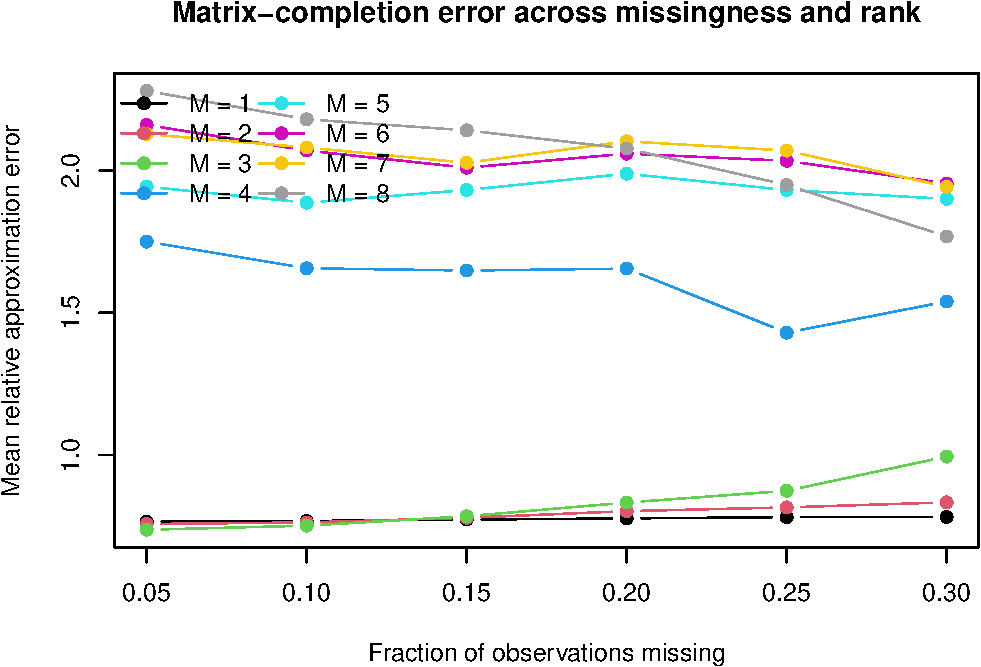
\includegraphics{ch12_exercises_files/figure-latex/matrix-completion-plot-1} \end{center}

The expected pattern is that error increases as the missing fraction
grows: with more entries hidden, the algorithm has less information from
which to recover the latent structure. Increasing \(M\) often lowers
error at first because the approximation is more flexible. However, the
benefit can flatten or reverse when a high-rank approximation starts
fitting idiosyncratic noise rather than the stable structure shared
across the matrix.

The exact ranking of the curves is an empirical result, not a theorem.
It depends on the random masks, the tolerance, and the structure of the
data. The 10 repetitions reduce the chance that one unusually easy or
difficult mask determines the conclusion.

\subsection{Convergence diagnostics}\label{convergence-diagnostics}

The function was also required to track iteration count. We summarize
the average number of iterations and the fraction of fits that reached
the specified tolerance.

\begin{Shaded}
\begin{Highlighting}[]
\NormalTok{iteration\_summary }\OtherTok{\textless{}{-}} \FunctionTok{aggregate}\NormalTok{(}
\NormalTok{  iterations }\SpecialCharTok{\textasciitilde{}}\NormalTok{ missing\_fraction }\SpecialCharTok{+}\NormalTok{ M,}
  \AttributeTok{data =}\NormalTok{ experiment\_results,}
  \AttributeTok{FUN =}\NormalTok{ mean}
\NormalTok{)}

\NormalTok{convergence\_summary }\OtherTok{\textless{}{-}} \FunctionTok{aggregate}\NormalTok{(}
\NormalTok{  converged }\SpecialCharTok{\textasciitilde{}}\NormalTok{ missing\_fraction }\SpecialCharTok{+}\NormalTok{ M,}
  \AttributeTok{data =}\NormalTok{ experiment\_results,}
  \AttributeTok{FUN =}\NormalTok{ mean}
\NormalTok{)}

\FunctionTok{list}\NormalTok{(}
  \AttributeTok{mean\_iterations =}\NormalTok{ iteration\_summary,}
  \AttributeTok{fraction\_converged =}\NormalTok{ convergence\_summary}
\NormalTok{)}
\end{Highlighting}
\end{Shaded}

\begin{verbatim}
## $mean_iterations
##    missing_fraction M iterations
## 1              0.05 1        8.8
## 2              0.10 1       11.4
## 3              0.15 1       14.9
## 4              0.20 1       21.2
## 5              0.25 1       25.6
## 6              0.30 1       40.9
## 7              0.05 2       13.1
## 8              0.10 2       20.9
## 9              0.15 2       34.3
## 10             0.20 2       68.5
## 11             0.25 2       98.2
## 12             0.30 2      229.1
## 13             0.05 3       20.8
## 14             0.10 3       31.0
## 15             0.15 3       90.6
## 16             0.20 3      215.0
## 17             0.25 3      347.0
## 18             0.30 3      455.3
## 19             0.05 4      442.3
## 20             0.10 4      477.2
## 21             0.15 4      490.9
## 22             0.20 4      500.0
## 23             0.25 4      500.0
## 24             0.30 4      500.0
## 25             0.05 5      500.0
## 26             0.10 5      500.0
## 27             0.15 5      500.0
## 28             0.20 5      500.0
## 29             0.25 5      500.0
## 30             0.30 5      500.0
## 31             0.05 6      500.0
## 32             0.10 6      500.0
## 33             0.15 6      500.0
## 34             0.20 6      500.0
## 35             0.25 6      500.0
## 36             0.30 6      500.0
## 37             0.05 7      500.0
## 38             0.10 7      500.0
## 39             0.15 7      500.0
## 40             0.20 7      500.0
## 41             0.25 7      500.0
## 42             0.30 7      500.0
## 43             0.05 8      500.0
## 44             0.10 8      500.0
## 45             0.15 8      500.0
## 46             0.20 8      500.0
## 47             0.25 8      500.0
## 48             0.30 8      500.0
## 
## $fraction_converged
##    missing_fraction M converged
## 1              0.05 1       1.0
## 2              0.10 1       1.0
## 3              0.15 1       1.0
## 4              0.20 1       1.0
## 5              0.25 1       1.0
## 6              0.30 1       1.0
## 7              0.05 2       1.0
## 8              0.10 2       1.0
## 9              0.15 2       1.0
## 10             0.20 2       1.0
## 11             0.25 2       1.0
## 12             0.30 2       0.9
## 13             0.05 3       1.0
## 14             0.10 3       1.0
## 15             0.15 3       1.0
## 16             0.20 3       0.8
## 17             0.25 3       0.6
## 18             0.30 3       0.2
## 19             0.05 4       0.2
## 20             0.10 4       0.2
## 21             0.15 4       0.1
## 22             0.20 4       0.0
## 23             0.25 4       0.0
## 24             0.30 4       0.0
## 25             0.05 5       0.0
## 26             0.10 5       0.0
## 27             0.15 5       0.0
## 28             0.20 5       0.0
## 29             0.25 5       0.0
## 30             0.30 5       0.0
## 31             0.05 6       0.0
## 32             0.10 6       0.0
## 33             0.15 6       0.0
## 34             0.20 6       0.0
## 35             0.25 6       0.0
## 36             0.30 6       0.0
## 37             0.05 7       0.0
## 38             0.10 7       0.0
## 39             0.15 7       0.0
## 40             0.20 7       0.0
## 41             0.25 7       0.0
## 42             0.30 7       0.0
## 43             0.05 8       0.0
## 44             0.10 8       0.0
## 45             0.15 8       0.0
## 46             0.20 8       0.0
## 47             0.25 8       0.0
## 48             0.30 8       0.0
\end{verbatim}

A larger missing fraction can require more iterations because the
observed entries provide a weaker anchor for the missing values. If a
fit reaches \texttt{max\_iter} before the tolerance is met, that is not
automatically a failure: it is a diagnostic signal that the chosen
tolerance or rank may require more iterations, or that the alternating
SVD updates are converging slowly.

\section{Conclusion}\label{conclusion}

Exercise 4 illustrates how a precise definition of cluster distance
controls the geometry of a dendrogram. Complete linkage cannot assign a
lower distance to a pair of clusters than single linkage because a
maximum cannot be below a minimum. For singleton clusters, both
definitions reduce to the same pairwise distance.

Exercise 11 turns the low-rank idea into an algorithm. Missing entries
are initialized, a rank-\(M\) SVD approximation is computed, and only
the missing entries are replaced. The observed entries remain fixed
throughout. The experiment then evaluates the method honestly on entries
that were hidden from it, across nested missingness levels, ranks
\(M=1\) through \(8\), and 10 random repetitions. This separates
algorithmic convergence from predictive approximation quality and makes
the effect of missingness visible.

\end{document}
